\documentclass[nobib]{tufte-handout}

\title{Föreläsning 6: Fortsättning på genererande funktioner $\cdot$ 1MA020}

\author[Vilhelm Agdur]{Vilhelm Agdur\thanks{\href{mailto:vilhelm.agdur@math.uu.se}{\nolinkurl{vilhelm.agdur@math.uu.se}}}}

%\date{15 januari 2023}


%\geometry{showframe} % display margins for debugging page layout

\usepackage{graphicx} % allow embedded images
  \setkeys{Gin}{width=\linewidth,totalheight=\textheight,keepaspectratio}
  \graphicspath{{graphics/}} % set of paths to search for images
\usepackage{amsmath}  % extended mathematics
\usepackage{booktabs} % book-quality tables
\usepackage{units}    % non-stacked fractions and better unit spacing
\usepackage{multicol} % multiple column layout facilities
\usepackage{lipsum}   % filler text
\usepackage{fancyvrb} % extended verbatim environments
  \fvset{fontsize=\normalsize}% default font size for fancy-verbatim environments

\usepackage{color,soul} % Highlights for text

% Standardize command font styles and environments
\newcommand{\doccmd}[1]{\texttt{\textbackslash#1}}% command name -- adds backslash automatically
\newcommand{\docopt}[1]{\ensuremath{\langle}\textrm{\textit{#1}}\ensuremath{\rangle}}% optional command argument
\newcommand{\docarg}[1]{\textrm{\textit{#1}}}% (required) command argument
\newcommand{\docenv}[1]{\textsf{#1}}% environment name
\newcommand{\docpkg}[1]{\texttt{#1}}% package name
\newcommand{\doccls}[1]{\texttt{#1}}% document class name
\newcommand{\docclsopt}[1]{\texttt{#1}}% document class option name
\newenvironment{docspec}{\begin{quote}\noindent}{\end{quote}}% command specification environment

\include{mathcommands.extratex}

\begin{document}

\definecolor{darkgreen}{rgb}{0.0627, 0.4588, 0.1451}

\maketitle% this prints the handout title, author, and date

\begin{abstract}
\noindent
Vi fortsätter förra föreläsningens diskussion om genererande funktioner, och ger fler exempel och sätt att använda sådana för att lösa kombinatoriska problem.
\end{abstract}

\section{Antal lösningar till en ekvation, med begränsningar}

I slutet på förra föreläsningen studerade vi antalet lösningar till ekvationen
$$x_1 + x_2 + x_3 + x_4 + x_5 = k$$
om vi kräver att alla $x_i$ är ickenegativa heltal. Det var ett första exempel på en mer generell kategori av problem med att räkna lösningar på ekvationer. Låt oss börja med ett lite mer invecklat problem:

\begin{example}
    Hur många lösningar finns det till
    $$x_1 + x_2 + x_3 + x_4 = k$$
    om vi kräver att alla $x_i$ är ickenegativa heltal, men också kräver att $x_2$ är jämnt, att $x_3 \leq 10$, och $x_4$ är udda?

    Låt, för varje $k$, $a_k$ vara antalet sådana lösningar.
    Låt sedan $a_k^1$ vara antalet lösningar till $x_1 = k$ i ickenegativa heltal $x_1$,
    $a_k^2$ vara antalet lösningar till $x_2=k$ i ickenegativa jämna heltal,
    $a_k^3$ vara antalet lösningar till $x_3=k$ i heltal mellan $0$ och $10$,
    och $a_k^4$ vara antalet lösningar till $x_4 = k$ i udda heltal.

    Precis som i förra exemplet studerar vi nu faltningen av dessa fyra följder, och ser att
    $$(a^1 * a^2 * a^3 * a^4)_k = \sum_{\substack{k_1, k_2, k_3, k_4\geq 0\\k_1 + k_2 + k_3 + k_4 = k}} a_{k_1}^1a_{k_2}^2a_{k_3}^3a_{k_4}^4 = a_k$$
    eftersom $a_{k_1}^1a_{k_2}^2a_{k_3}^3a_{k_4}^4$ är en produkt av ettor och nollor -- att $k_1 + k_2 + k_3 + k_4 = k$ garanteras av definitionen av faltning, och sedan är varje term i produkten ett om värdet på $k_i$ är tillåtet av våra begränsningar, och noll annars. Så produkten är ett om summan är korrekt och varje enskild begränsning är uppfylld.

    Så precis som i förra exemplet kan vi få fram genererande funktionen för $a_k$, följden vi faktiskt är intresserade av, genom att plocka fram den genererande funktionen för de enklare följderna.

    Vad genererande funktionen för $a^1$ är vet vi sedan innan -- den är bara en följd av ettor, så dess genererande funktion blir $\frac{1}{1-x}$. Likaledes vet vi sedan innan att följden av $n$ stycken ettor och sedan nollor har genererande funktion $\frac{1 - x^{n+1}}{1-x}$, så genererande funktionen för $a^3$ blir $\frac{1 - x^{11}}{1-x}$.

    Däremot för $a^2$ behöver vi räkna ut något nytt, nämligen den genererande funktionen för följden $1,0,1,0,1,\ldots$, indikatorfunktionen av de jämna talen. Så vi får skriva att
    \begin{align*}
        F_{a^2}(x) &= \sum_{k=0}^{\infty} a^2_k x^k\\
        &= \sum_{\substack{k \geq 0\\k \in 2\Z}} x^k\\
        &= \sum_{i=0}^{\infty} x^{2i}\\
        &= \sum_{i=0}^{\infty} (x^2)^i
    \end{align*}
    och sista raden här kan vi känna igen som genererande funktionen av följden $(1,1,1,1,\ldots)$, \emph{utvärderad i} $x^2$. Så detta är lika med $\frac{1}{1-x^2}$.

    Så vad som återstår är alltså $a^4$, indikatorfunktionen för de udda talen. För att få fram dess genererande funktion kan vi använda vad vi just gjorde för de jämna talen:
    \begin{align*}
        F_{a^4}(x) &= \sum_{k=0}^{\infty} a_k x^k\\
        &= \sum_{\substack{k \geq 1\\k\text{ udda}}} x^k\\
        &= x\sum_{\substack{k \geq 1\\k\text{ udda}}} x^{k-1}\\
        &= x\sum_{\substack{k \geq 0\\k \in 2\Z}} x^k\\
        &= \frac{x}{1 - x^2}.
    \end{align*}

    Så, om vi använder att genererande produkten av en faltning är produkten av de genererande funktionerna, ser vi att
    \begin{align*}
        F_a(x) &= \left(\frac{1}{1-x}\right)\left(\frac{1-x^{11}}{1-x}\right)\left(\frac{1}{1-x^2}\right)\left(\frac{x}{1-x^2}\right)\\
        &= \frac{x(1 - x^{11})}{(1-x)^2(1-x^2)^2}
    \end{align*}
    och ber vi vårt favorit-CAS\sidenote[][]{\emph{Computer Algebra System}, alltså till exempel \emph{WolframAlpha} eller något av dess öppna alternativ, såsom \emph{Sage}.} att Taylorutvidga detta uttryck så får vi att
    $$F_a(x) = x + 2x^2 + 5x^3 + 8x^4 + 14x^5 + 20x^6 + 30x^7 + 40x^8 + \ldots$$
    så att följden av antalet lösningar är
    $$0,1,2,5,8,14,20,30,40,55,70,91,111,138,163,\ldots.$$
\end{example}

\begin{example}
  Vi vill räkna antalet lösningar $a_k$ till ekvationen
  $$2x_1 + x_2 + x_3 = k$$
  där alla $x_i$ är heltal, $x_2$ är en multipel av $6$, och talet $x_3$ kan vara antingen rött eller blått.\sidenote[][]{Vi ser alltså, för $k = 6$, alla dessa som godtagbara distinkta lösningar:
  $$x_1 = 1, x_2 = 0, x_3 = \textcolor{blue}{4}, \qquad x_1 = 1, x_2 = 0, x_3 = \textcolor{red}{4},$$
  $$x_1 = 2, x_2 = 0, x_3 = \textcolor{blue}{2}, \qquad x_1 = 0, x_2 = 6, x_3 = \textcolor{red}{0}.$$}

  Vi börjar med att göra variabelbytet $y_1 = 2x_1$, och vill alltså nu ha lösningar till $y_1 + x_2 + x_3 = k$, med begränsningen att $y_1$ är jämnt. Det här förändrar så klart inte antalet lösningar, bara gör det lättare för oss att tillämpa vår metod.

  Vi tillämpar samma metod som i förra exemplet, och låter $a^1_k$ vara antalet lösningar till $y_1 = k$ med $y_1$ jämnt, $a^2_k$ vara antalet lösningar till $x_2 = k$ med $x_2$ delbart med $6$, och $a^3_k$ vara antalet lösningar till $x_3 = k$ med $x_3$ färgat antingen rött eller blått. Faltningen blir då 
  $$(a^1 * a^2 * a^3)_k = \sum_{\substack{k_1, k_2, k_3 \geq 0\\k_1+k_2+k_3 = k}} a^1_{k_1}a^2_{k_2}a^3_{k_3} = a_k.$$

  Vi fortsätter precis som innan med att räkna ut den genererande funktionen för varje av våra följder. För $a^1$ vet vi redan vad genererande funktionen för indikatorfunktionen av de jämna talen är, nämligen $\frac{1}{1-x^2}$. 
  
  För $a^2$ kan vi använda samma metod som vi använde för de jämna talen för att se att
  \begin{align*}
    F_{a^2}(x) &= \sum_{k=0}^{\infty} a^2_k x^k = \sum_{\substack{k \geq 0\\k \in 6\Z}} x^k\\
    &= \sum_{i=0}^{\infty} x^{6i} = \sum_{i=0}^{\infty} (x^6)^i
  \end{align*}
  så att $F_{a^2}(x) = \frac{1}{1-x^6}$.

  För $a^3$ så blir denna helt enkelt en följd av bara tvåor, eftersom vi har två val för färg för varje tal, och kan välja vilket tal som helst. Så vi ser att
  $$F_{a^3}(x) = \sum_{k=0}^{\infty} 2x^k = 2\frac{1}{1-x}.$$

  Sammantaget har vi alltså att
  $$F_a(x) = \left(\frac{1}{1-x^2}\right)\left(\frac{1}{1-x^6}\right)\left(\frac{2}{1-x}\right) = \frac{2}{(1-x)(1-x^2)(1-x^6)}$$
  vilket vi kan Taylorutvidga i vårt favoritprogram och få att\sidenote[][]{Vi ser ju ett tydligt mönster här av att $a_{2k} = a_{2k+1}$. Kan du förklara varför detta måste vara fallet, baserat på våra begränsningar av variablerna?}
  \begin{align*}
    F_a(x) &= 2 + 2 x + 4 x^2 + 4 x^3 + 6 x^4 + 6 x^5 + 10 x^6 + 10 x^7\\
    & + 14 x^8 + 14 x^9 + 18 x^{10} + 18 x^{11} + 24 x^{12} + 24 x^{13}\\
    & + 30 x^{14} + 30 x^{15} + 36 x^{16} + 36 x^{17} + 44 x^{18} + \ldots.
  \end{align*}
\end{example}

\begin{example}
  Antag att vi har ett schackbräde med $2\times n$ rutor, och vi vill täcka det med brickor av formen $2\times 1$ eller $1\times 2$. Hur många sätt kan vi göra detta på?

  \begin{marginfigure}
    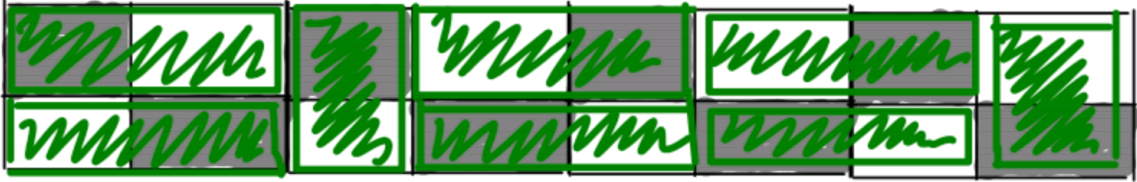
\includegraphics{graphics/checkerboard_tiling.png}
    \caption{Ett sätt att göra detta då $n=8$. Figur tagen ur förra årets anteckningar.}
  \end{marginfigure}

  Låt $t_n$ vara antalet sätt vi kan täcka vårt schackbräde. Vi vill hitta en rekursion för detta antal. Vi ser enkelt att det finns ett enda sätt att göra det för $n=1$ -- bara en bricka får plats -- så $t_1 = 1$. För $n=2$ finns det två sätt, antingen lägger vi dem horisontellt eller vertikalt, så $t_2 = 2$.

  \begin{marginfigure}
    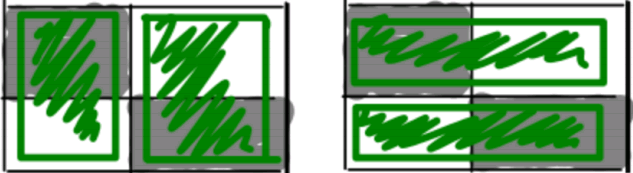
\includegraphics{graphics/checkerboard_tiling_n_2.png}
    \caption{De två sätten att göra det på då $n=2$. Figur från förra årets föreläsningsanteckningar.}
  \end{marginfigure}

  Om vi vill skapa oss en täckning av en $2\times n$-bräda, för något $n > 2$, kan vi göra på två sätt:
  \begin{itemize}
    \item Vi börjar med en täckning av en $2\times(n-1)$-bräda, och lägger till en till bricka vertikalt.
    \item Vi börjar med en täckning av en $2\times(n-2)$-bräda, och lägger till två till brickor horisontellt.
  \end{itemize}

  Att varje täckning av en $2\times n$-bräda kan skapas på detta vis är enkelt att se -- antingen är den sista kolumnen täckt av en vertikal bricka, i vilket fall vi skapade täckningen på första viset, eller så är den täckt av två horisontella brickor, i vilket fall vi skapade den på det andra sättet.

  Alltså har vi funnit följande rekursion för antalet täckningar
  $$t_0 = 0, t_1 = 1, t_2 = 2, \quad t_n = t_{n-1} + t_{n-2} \, \forall n > 2$$
  som ju är extremt lik den vi har för Fibonaccitalen, så vi kan finna en genererande funktion och sluten form på precis samma vis som i det fallet.
\end{example}

\section{Övningar}

\begin{xca}
  Hur många heltalslösningar till ekvationen
  $$x_1 + x_2 + x_3 = 578$$
  finns det,\sidenote[][-2cm]{Om ni väl har hittat genererande funktionen för antalet lösningar när vi ersatt $578$ med $k$, så kan ni enkelt få fram svaret med följande kod till \emph{WolframAlpha}:
  $$\mathtt{SeriesCoefficient}[f, \{x,0,578\}]$$
  där $f$ då är genererande funktionen ni funnit. Att ange den genererande funktionen och säga att ni sedan plockade fram rätt koefficient ur den med hjälp av ett CAS är den förväntade metoden här.} om vi kräver att
  \begin{itemize}
    \item $x_1 \geq -7$,\sidenote[][]{Ledtråd: Gör ett variabelbyte till $y_1$ för att få den vanliga begränsningen att $y_1 \geq 0$.}
    \item $x_2 \geq 0$ är ett jämnt tal,
    \item och $x_3 \geq 0$ kan vara vilket tal som helst, men om det är jämnt kan det vara rött eller blått, och om det är udda kan det vara gult, grönt, eller lila. 
  \end{itemize}
\end{xca}

%\bibliography{references}
%\bibliographystyle{plainnat}

\end{document}
